\capitulo{4}{Metodología}

Los modelos y simulaciones analizados a continuación simplifican el funcionamiento del sistema glucorregulatorio de nuestro organismo. Su finalidad es estudiar el comportamiento y efecto de dicho sistema, quedando fuera de este estudio, la definición de nuevos criterios para establecer rangos o parámetros específicos de la interacción entre la glucosa y la insulina. De esta forma, el modelado de la glucosa permite observar cómo afectan ciertas variables a su comportamiento.

\section{Descripción de los datos}
Se presenta un estudio que modela el comportamiento de la glucosa e insulina para pacientes no diabéticos y diabéticos. Se han seleccionado para ello, dos pares de valores de glucosa e insulina basal, uno para cada tipo de paciente. Esta elección ha sido realizada teniendo en cuenta los rangos diabéticos mostrados en la Tabla  \ref{tab:rangos_diabeticos}, así como teniendo en cuenta lo mencionado por Jaime Carrillo Moreno y otros en \cite{carrillo2021long}. De esta manera, se considera que representan adecuadamente las características propias de su grupo.

La glucosa se mide en mg /dL. La inclusión de esta variable en el modelo se realiza en mmol/L, lo que implica el uso de factores de conversión. La relación entre ambas unidades se basa en que 1 mmol/L = 18 mg/dL.
La insulina se mide en mU /L.
Los parámetros de los modelos empleados en el análisis han sido seleccionados en base a su uso en estudios previos, garantizando su validez debido a que han demostrado ser efectivos y relevantes en investigaciones anteriores sobre diabetes y sus marcadores.

Se presentan en la siguientes tablas, Tabla \ref{tab:valores_no_diabetico} y Tabla \ref{tab:valores_diabetico}, los valores estimados para el paciente no diabético y para el paciente diabético.

\begin{table}[htbp]
    \centering
    \caption{Valores basales estimados para el paciente base.}
    \begin{tabular}{|c|c|c|}
        \hline
          & Valor\\
        \hline
        Gb & 81 mg/dL \\
        Ib & 12 mU/L  \\
        \hline
    \end{tabular}
    \label{tab:valores_no_diabetico}
\end{table}
\begin{table}[htbp]
    \centering
    \caption{Valores basales estimados para el paciente diabético.}
    \begin{tabular}{|c|c|c|}
        \hline
          & Valor\\
        \hline
        Gb & 126 mg/dL \\
        Ib & 10 mU/L  \\
        \hline
    \end{tabular}
    \label{tab:valores_diabetico}
\end{table}

\subsection{Parámetros glucémicos empleados en el análisis}

Los valores asignados a los parámetros incluidos en los modelos para este estudio son los establecidos por \cite{fisher1991semiclosed}.

\begin{table}[htbp]
    \centering
    \caption{Valores de los paráemtros glucémicos de los modelos de la glucosa.}
    \begin{tabular}{|c|c|c|}
        \hline
        Parámetro & Valor& Unidad \\
        \hline
        $p_1$ & 0.028 & $min^{-1}$ \\
        $p_2$ & 0.025 & $min^{-1}$ \\
        $p_3$ & 0.000013 &  $min^{-2} (\mu UI / mL)$\\
        $p_6$ & 0.003349 & $min^{-1}$ \\
        n & 5/54 & $min^{-1}$ \\
        $V_i$ & 12 & L \\
        \hline
    \end{tabular}
    \label{tab:parametros_glucemicos}
\end{table}

\section{Modelo de Bergman}

Este modelo refleja el comportamiento del sistema glucorregulatorio de un \textbf{paciente sano}. El Modelo Mínimo se basa en la regla de balance de masa, que indica que la cantidad acumulada en un compartimento es exactamente:
\begin{equation}
acumulado = \text{cantidad entrada - cantidad salida + generado - consumido}
\label{eq:balance_masas}
\end{equation}
 Está formado por 2 ecuaciones diferenciales no lineales definidas por Bergman en \cite{bergman1979quantitative}, que estudian el comportamiento de la Glucosa G(t) y de la Insulina Activa X(t) a lo largo del tiempo \footnote{Información referente a este modelo ha sido comprendida gracias al desarrollo propuesto en \cite{perez2017analisis}}.
 Como se ha comentado antes, se remarca la importancia de la diferencia entre estas dos variables. Mientras que \textit{insulina activa} es la parte de insulina lista para ser utilizada por el cuerpo para regular los niveles de azúcar en sangre, la \textit{insulina normal} es la forma 'inactiva' o almacenada en la hormona. Cuando es necesario, el organismo convierte la insulina normal en activa para cumplir sus funciones. 
\begin{align}
    \frac{dG(t)}{dt}= -p_1 (G(t) - G_b) - X(t)G(t) , G(0) = Gb
    \label{eq:ecBergGluc}\\
    \frac{dX(t)}{dt}= -p_2 X(t) + p_3(I(t) - I_b),    X(0) = 0
    \label{eq:ecBergInsAc}
\end{align}

De esta manera, para la ecuación de la insulina activa X(t), el primer témino representa la velocidad a la que esta se elimina en el cuerpo, mientras que la segunda parte de la ecuación representa la velocidad de transformación de insulina a insulina activa. La diferencia presente en esta parte de la ecuación refleja esta conversión. Si la concentración de insulina en un momento dado es mayor que la basal (I(t)>$I_b$), la diferencia será positiva, lo que supone un estímulo para la conversión a insulina activa. Por otro lado, si la insulina total es menor que la basal (I(t) <$I_b$), la diferencia será negativa, lo que supone un estímulo para la liberación de insulina en sangre, en vez de la conversión a insulina activa. 

El resto de variables y parámetros del modelo se definen a continuación:
\begin{enumerate}
    \item[-] $G_b$: valor de glucosa basal (cte.).
    \item[-] $I_b$: valor de insulina basal (cte.).
    \item[-] $p_1$: valor máximo inicial de la curva de interacción glucosa- insulina (cte.).
    \item[-] $p_2$: tasa disminución de glucosa en tejido por unidad de insulina (cte.).
    \item[-] $p_3$: tasa de incremento de glucosa después de la acción de la insulina (cte.). 
    \item[-] G(t): concentración de la glucosa en plasma.
    \item[-] I(t): concentración de la insulina en plasma.
    \item[-] X(t): concentración de la insulina activa en plasma.
\end{enumerate}

\subsection{Estabilidad del sistema}
\label{sec:est_estac}

Inicialmente se va a estudiar el comportamiento del modelo bajo condiciones estables, es decir, el sistema en equilibrio. Encontrar las concentraciones de glucosa e insulina en condiciones estables (sin cambios en entradas o en otras condiciones) es un punto clave para el análisis y la compresión de la regulación de la glucosa en el cuerpo humano. Este equilibrio se consigue hallando el estado estacionario del sistema estableciendo las derivadas de las variables a 0. En otras palabras, mediante este método se obtienen los puntos en los cuales las variables del sistema no cambian con el tiempo.
Partiendo de las ecuaciones iniciales, es posible hallar, por tanto, qué valores adoptan las variables G(t) y X(t) en equilibrio dados unos valores iniciales de Glucosa Basal (Gb) e Insulina Basal (Ib), y analizar así el comportamiento del sistema en condiciones estables.
Garantizando su invariabilidad con el tiempo, igualando a 0 \eqref{eq:ecBergGluc} y \eqref{eq:ecBergInsAc} :
\begin{align}
    0= -p_1 (G(t) - G_b) - X(t)G(t) \\
    0= -p_2 X(t) + p_3(I(t) - I_b) 
\end{align}
Para el caso base la condición es que X(0)=0. 
Por tanto, para la insulina activa:
\begin{align*}
    0= -p_2 X(0) + p_3(I(0) - I_b) \\
    0= -p_2 (0) + p_3(I(0) - I_b) \\
    0= p_3(I(0) - I_b) \\
    p_3 I_b= p_3 I(0) \\
    I_b = I(0) \\
\end{align*}

Por otro lado, para la glucosa:
\begin{align*}
    0= -p_1 (G(0) - G_b) - X(0)G(0) \\
    0= -p_1 (G(0) - G_b) - (0)G(0) \\
    0= -p_1 (G(0) - G_b) - 0 \\
    0= -p_1 (G(0) - G_b) \\
    p_1 G(0)= p_1 G_b \\
    G(0) = G_b \\
\end{align*}
Este comportamiento se refleja en la glucosa e insulina activa en la Figura \ref{fig:bergman_en_ayunas}.

\begin{figure}[htbp]
    \centering
    \begin{subfigure}[b]{0.9\linewidth} % Ancho ajustado al 90% del ancho de la línea
        \centering
        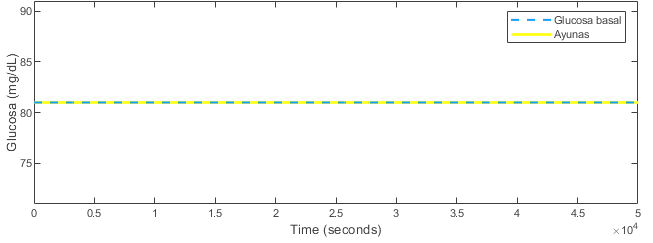
\includegraphics[width=\linewidth]{img/modelo_original/ayuno.png}
        \caption{Glucosa en ayuno.}
        \label{fig:bergman_ayunas_glucosa}
    \end{subfigure}
    
    \vspace{0.5cm} % Espacio vertical entre las subfiguras

    \begin{subfigure}[b]{0.9\linewidth} % Ancho ajustado al 90% del ancho de la línea
        \centering
        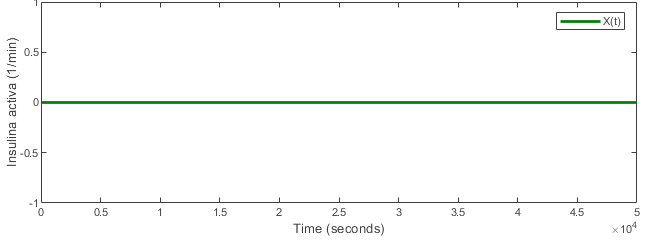
\includegraphics[width=\linewidth]{img/modelo_original/ins_act_ayuno.png}
        \caption{Insulina activa en ayuno.}
        \label{fig:bergman_ayunas_insulina_activa}
    \end{subfigure}
    
    \caption{Comportamiento de la glucosa e insulina activa para una situación en equilibrio, sin perturbaciones. Fuente propia.}
    \label{fig:bergman_en_ayunas}
\end{figure}


De esta forma se define el comportamiento de la glucosa en el organismo para condiciones estables o equilibrio.
Mientras no se reciba ninguna perturbación, la insulina no varía con respecto a la insulina basal, así como la glucosa no varía respecto de la glucosa basal. La insulina activa, por su parte, se ve obligada a mantenerse en 0, pues la insulina I(t) no experimenta ninguna variación.

\subsection{Modelado dinámico de la insulina}

Para el Modelo de Bergman, la insulina no se encuentra modelada, pues se trataba como un vector de medidas a lo largo del tiempo obtenidas tras una ingesta, ya que el modelo estaba pensado para para la prueba IVGTT.

En esta sección, se modifica el tratamiento de la insulina I(t) dentro del modelo, evolucionando de una constante fija a una ecuación que varía con el tiempo. Esta actualización tiene como objetivo emular de manera más precisa el comportamiento dinámico del páncreas en la regulación de los niveles de insulina. Esta implementación de una función variable con el tiempo, obtenida de \cite{alonso2014modelos}, tiene como finalidad reflejar mejor la fisiología del páncreas y su respuesta a los niveles de glucosa.
\begin{equation}
    \frac{dI(t)}{dt} = p_6 (G(t)-p_5)^+ t -n(I(t)+Ib), Ib(0)=0
    \label{eq:insulina_variable}
\end{equation}
La ecuación \eqref{eq:insulina_variable}, que se une al sistema formado por \eqref{eq:ecBergGluc} y \eqref{eq:ecBergInsAc}  modela el comportamiento del páncreas en relación con la liberación de insulina en respuesta a los niveles de glucosa en la sangre, concretamente el término:
\begin{equation}
    Páncreas (t)= (G(t)-p_5)^+ t 
    \label{eq:pancreas}
\end{equation}
Este término se conoce como la “parte positiva” de la diferencia G(t) - $p_5$, donde $p_6$ es la constante de proporcionalidad en la tasa de cambio en la insulina. Mientras que $p_6$ y n se encuentran definidos en la Tabla \ref{tab:parametros_glucemicos}, el parámetro $p_5$ es un valor específico que define el punto en el cual el nivel de glucosa en la sangre se considera lo suficientemente alto como para activar la liberación de insulina por parte del páncreas. Este umbral es un límite crítico que determina si los niveles de glucosa en la sangre están por encima o por debajo del rango normal.
El umbral divide los niveles de glucosa en la sangre en dos regiones distintas: por encima y por debajo de $p_5$.
\begin{enumerate} \label{sec:p5}
    \item[-] Si G(t) > $p_5$, el término \eqref{eq:pancreas}  tiene el valor de G(t) - $p_5$. Esto indica que el nivel de glucosa actual es superior del umbral de glucosa establecido, y por tanto, se debe liberar insulina para reducir los niveles de glucosa. Cuando G(t) = $p_5$, finalizará la liberación.
    \item[-] Si G(t) <= $p_5$, el término \eqref{eq:pancreas} tiene el valor de 0, pues la glucosa no es suficientemente alta como para que sea necesario liberar insulina para reducirla.
\end{enumerate}

Para las siguientes gráficas de Figura \ref{fig:bergman_p5_base}, se observa el comportamiento de la glucosa bajo la liberación de la insulina por parte del páncreas. La raya vertical delimita el umbral de $p_5$. Para este caso, se comienza con una glucosa de 144 mg/gL y un $p_5$ = 117 mg/dL, por lo que G(t) > $p_5$. Cuando $p_5$ se iguala a G(t), el páncreas deja de liberar insulina y su gráfica experimenta una caida hasta volver al nivel basal.
\clearpage
\begin{figure}[htbp]
    \centering
    \begin{subfigure}[b]{0.9\linewidth} % Ancho ajustado al 90% del ancho de la línea
        \centering
        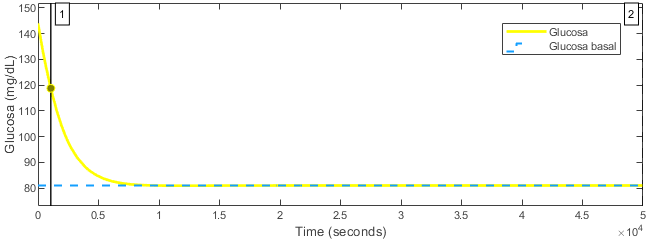
\includegraphics[width=\linewidth]{img/modelo_original/p5_base_gluc.PNG}
        \caption{Glucosa con umbral p5.}
        \label{fig:bergman_p5_glucosa}
    \end{subfigure}
    
    \vspace{0.5cm} % Espacio vertical entre las subfiguras

    \begin{subfigure}[b]{0.9\linewidth} % Ancho ajustado al 90% del ancho de la línea
        \centering
        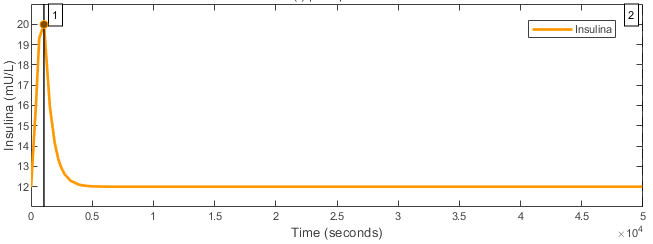
\includegraphics[width=\linewidth]{img/modelo_original/p5_base_ins.PNG}
        \caption{Insulina con umbral p5.}
        \label{fig:bergman_p5_insulina}
    \end{subfigure}
    
    \caption{Efecto de la selección de un umbral p5 determinado para la liberación de insulina. Fuente propia.}
    \label{fig:bergman_p5_base}
\end{figure}



\subsection{Descripción de los parámetros}

El Modelo de Bergman cuenta con 3 parámetros clave para la representación del funcionamiento del sistema glucorregulatorio del organismo: $p_1$, $p_2$ y $p_3$.
\begin{enumerate}
    \item $p_1$ es la tasa de eliminación de la glucosa, y sus valores para un paciente normal oscilan en el rango entre 0.02 – 0.05 $min^{-1}$. 
    
    Un paciente diabético verá disminuido su valor de $p_1$, encontrándose en el límite inferior del rango, incluso quedando por debajo de él.
    
    \item $p_2$ es la tasa de insulina activa, y su rango es el mismo que en el anterior caso (0.02 - 0.05 $min^{-1}$). 
   
    En ayuno, $p_2$  tiende a acercarse al extremo inferior del rango, mientras que, tras la ingesta, el valor aumenta. Para pacientes diabéticos, debido a la disminución de la producción de insulina, así como la disminución de sensibilidad de los tejidos a la insulina, $p_2$  disminuye notablemente.
    
    \item $p_3$ constituye el coeficiente de transformación de insulina a insulina activa, y sus valores oscilan entre $10^{-5}$ y $10^{-6}
    L/mU$ $min ^2$. 
    
    Para pacientes diabéticos, concretamente para DM2, debido a la resistencia a la insulina, el cuerpo produce más insulina, lo que se traduce en un aumento de $p_3$.
\end{enumerate}

De la misma forma, se ha considerado realizar un análisis propio e independiente de estos parámetros, mediante el estudio de su variación, para comprobar que los rangos son correctos, así como que los valores asignados a cada parámetro son adecuados. Los valores modificados se encuentran en el anexo.

\section{Modelo de Bergman Modificado}
\label{sec:indicar_n}
El modelo matemático estudiado en la sección anterior pierde su eficacia cuando el sistema glucosa - insulina ve alterado su comportamiento. En particular, en pacientes diabéticos tipo 1, cuando el páncreas no puede generar insulina, la ecuacion (\ref{eq:pancreas}) no es adecuada. 
Se introduce un modelo modificado,  obtenido en \cite{zamarron2021modelos}, que incluye la insulina exógena U. Este nuevo comportamiento se representa mediante una nueva ecuación para el Modelo de Bergman, que adopta una nueva implementación para I(t).
\begin{align}
    \frac{dG(t)}{dt}= -p_1 (G(t) - G_b) - X(t)G(t), G(0)=Gb \\ \label{eq:glucosa_mod_mod}
    \frac{dX(t)}{dt}= -p_2 X(t) + p_3(I(t) - I_b), X(0) = 0 \\
    \frac{dI(t)}{dt}= -n I(t) + \frac{U(t)}{Vi}, I(0) = Ib 
    \label{eq:ecBergMod}
\end{align}
Donde:
\begin{enumerate}
    \item[-] \textbf{1/n} es la constante de tiempo del sistema, e indica el tiempo que tarda la insulina en alcanzar el valor de la insulina exógena administrada (cte.). 
    \item[-] \textbf{Vi} es el volumen de distribución de insulina (cte.). 
    \item[-] \textbf{U(t)} es insulina exógena que se administra. 
\end{enumerate}

En la Figura \ref{fig:modificado_comportamiento_ayuno} se muestra el comportamiento de la glucosa e insulina para un paciente diabético tipo 1 en ayunas que no recibe administración de insulina exógena.

\begin{figure}[htbp]
    \centering
    \begin{subfigure}[b]{0.9\linewidth} % Ancho ajustado al 90% del ancho de la línea
        \centering
        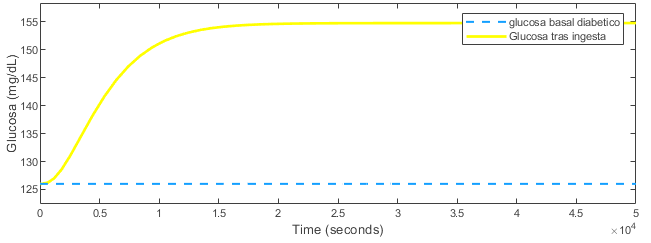
\includegraphics[width=\linewidth]{img/modelo_modificado/en_metodologia/glucosa_ayuno.png}
        \caption{Glucosa en ayuno diabético.}
        \label{fig:mod_ayuno}
    \end{subfigure}
    
    \vspace{0.5cm} % Espacio vertical entre las subfiguras

    \begin{subfigure}[b]{0.9\linewidth} % Ancho ajustado al 90% del ancho de la línea
        \centering
        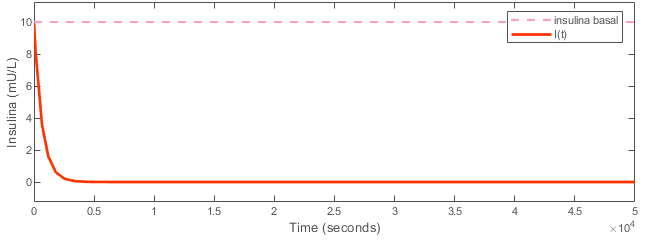
\includegraphics[width=\linewidth]{img/modelo_modificado/en_metodologia/insulina_ayuno.png}
        \caption{Insulina en ayuno diabético.}
        \label{fig:mode_ayuno_insu}
    \end{subfigure}
    
    \caption{Comportamiento de la glucosa e insulina en ayunas para un paciente diabético sin administración de insulina exógena. Fuente propia.}
    \label{fig:modificado_comportamiento_ayuno}
\end{figure}


Como se observa en las gráficas, cuando el paciente no recibe ninguna ingesta en ayuno, los niveles de glucosa en sangre se ven aumentados, pues la insulina presente en el organismo va disminuyendo (ya que hemos eliminado la insulina exógena). Los niveles de glucosa en sangre para el paciente no consiguen volver a la glucosa basal ($G_b$), pues no se está produciendo insulina en el organismo. Esta condición puede llevar a severas hiperglucemias.

\subsection{Dinámica del modelo ante una entrada: insulina exógena}

Como se ha visto anteriormente, la variable de entrada de insulina exógena U varía dependiendo del tipo de acción que induce en el organismo.
Debido a que la modelización de estos tipos de insulina y su efecto en el organismo es una labor compleja (principalmente por su variación a lo largo del tiempo), este estudio se centrará en el efecto causado por la administración de insulina en cuanto a su cantidad, y, en menor medida, respecto a su hora de administración.
1 IU de insulina humana equivale aproximadamente a 0.0347 mg. Esto se basa en la potencia biológica de la insulina, donde 1 mg de insulina tiene una actividad de aproximadamente 28.8 IU \footnote{Se establece esta relación aproximada en \cite{cima_insulina}, donde se aporta el cálculo específico para la insulina humana anhidra.}.

Para el caso basal, donde no se presentan perturbaciones externas, se espera que los niveles de glucosa e insulina permanezcan constantes en el organismo. Sin embargo, esta premisa no se cumple en sistemas glucorregulatorios alterados, los cuales exhiben una variabilidad en el nivel de glucosa basal, mostrando un aumento constante en su concentración. Se calcula, para el paciente diabético (Tabla \ref{tab:valores_diabetico}) la insulina exógena necesaria para volver a sus niveles estables de glucosa. Partiendo del estado estacionario (estudiado en la Sección \ref{sec:est_estac}), donde se ha obtenido que G(0) = Gb y que I(0)=Ib, igualamos a cero la tercera ecuación del sistema (\ref{eq:ecBergMod}), la insulina.
\begin{align}
    0= -n I(t) + \frac{U(t)}{Vi}
\end{align}
Teniendo en cuenta que I(0) = Ib:
\begin{align}
    0= -n Ib + \frac{U(t)}{Vi}
    n Ib = \frac{U(t)}{Vi}
    U(t) = n Ib Vi
\end{align}
\label{sec:insulina_calculo}
Para este paciente  se obtiene una U(t) = 0.185 mU/L. En la Figura \ref{fig:modificado_comportamiento_insulina_exogena} se muestra el efecto de la adición de esta insulina en el paciente.
\label{sec:dosis_insu_base}
\clearpage
\begin{figure}[htbp]
    \centering
    \begin{subfigure}[b]{0.9\linewidth} % Ancho ajustado al 90% del ancho de la línea
        \centering
        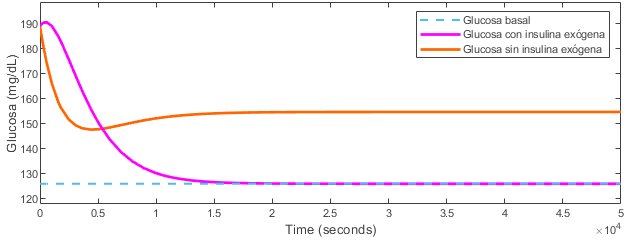
\includegraphics[width=\linewidth]{img/modelo_modificado/en_metodologia/con_insulina_glucosa.png}
        \caption{Glucosa con insulina exógena.}
        \label{fig:mod_ayuno}
    \end{subfigure}
    
    \vspace{0.5cm} % Espacio vertical entre las subfiguras

    \begin{subfigure}[b]{0.9\linewidth} % Ancho ajustado al 90% del ancho de la línea
        \centering
        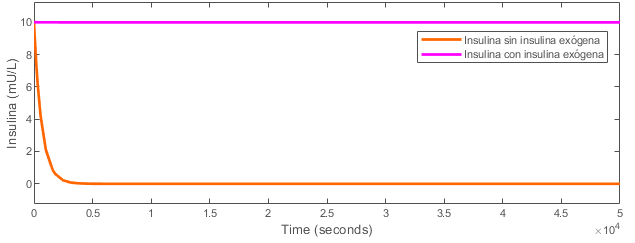
\includegraphics[width=\linewidth]{img/modelo_modificado/en_metodologia/con_insulina_insulina.png}
        \caption{Insulina con insulina exógena.}
        \label{fig:mode_ayuno_insu}
    \end{subfigure}
    
    \caption{Comparación del comportamiento de la glucosa e insulina tras una ingesta sin y con insulina exógena (U=0.185 mg). Fuente propia.}
    \label{fig:modificado_comportamiento_insulina_exogena}
\end{figure}


Se pretende abordar un segundo escenario, donde se busca encontrar el efecto en el organismo de la administración de insulina de acción rápida. Aunque esta representación puede no ser completamente precisa, se intentará diferenciar el impacto de la inyección de insulina de acción rápida en el organismo de manera tentativa, considerando su efecto inmediato en la reducción de los niveles de glucosa en sangre frente a otras formas de insulina con diferentes perfiles de acción. Para realizar esta aproximación se emplea la información relacionada con duración, pico y efecto mencionada en la Sección \ref{sec:ins_ex}, y bloques \textit{Rampa} de Simulink, cuya pendiente P se calcula:
\clearpage
\begin{small}
\begin{align}
    P ascendente = \frac{Insulina Exógena Final-Insulina Exógena Inicial}{tiempo}= \\
    \frac{Insulina Exógena Máxima-Insulina Exógena Mínima}{tiempo}\\
    P descendiente = \frac{Insulina Exógena Final-Insulina Exógena Inicial}{tiempo}=\\
    \frac{Insulina Exógena Mínima-Insulina Exógena Máxima}{tiempo}\\
\end{align}
\end{small}

\subsection{Incorporación dinámica de perturbaciones}

\subsubsection{\underline{La ingesta}}

La variable de ingesta ha sido añadida en el modelo de regulación glucémica de forma similar que en \cite{tarin2021modelo} para capturar los efectos de la alimentación en los niveles de glucosa en sangre. La ingesta D(t) se refleja en la ecuación de la glucosa G(t), presentando una relación directamente proporcional con esta, pues, a mayor cantidad de ingesta, mayores se esperan que sean los niveles de glucosa en sangre. Se modifica la ecuación de la glucosa del sistema (\ref{eq:glucosa_mod_mod}) para obtener:
\begin{align}
    \frac{dG(t)}{dt}= -p_1 (G(t) - G_b) - X(t)G(t)+D(t), G(0)=Gb \label{eq:glucosa_ingesta_bergm}
\end{align}

La ecuación particular para la ingesta, que simula un decaimiento exponencial de la ingesta una vez realizada, es denotada como D(t) y se modela de la siguiente forma:
\begin{align}
    D(t)= \frac{D_g A_g t e^{-t/t_\text{max,i}}}{V_g t^{2}_\text{max,g}} \label{eq:ecu_ingesta}
\end{align}

$D_g$ es la cantidad de carbohidratos ingeridos, y representa la cantidad aproximada de ingesta del paciente, excluyendo de esta información el valor proteico o las grasas de la comida..
Esta ecuación describe la dinámica de la ingesta a lo largo del tiempo, considerando factores como la dosis, la amplitud, el tiempo de máximo, el volumen de distribución y su variación temporal (cuyos valores se encuentran incluidos en la Tabla \ref{tab:parametros_ingesta}).

La gráfica que genera esta ecuación se encuentra en la Figura \ref{fig:grafica_ingesta} para una cantidad de 50 gramos de carbohidratos. 

\begin{table}[htbp]
    \centering
    \caption{Valores de las constantes de la función ingesta.}
    \begin{tabular}{|c|c|c|}
        \hline
          & Valor & Unidad  \\
        \hline
        Ag & 0.8 & mmol/L \\
        Tmax,i & 55 & mU/L \\
        Tmax,g & 40 & $min^-1$ \\
        Vg & 13.79 & L \\
        \hline
    \end{tabular}
    \label{tab:parametros_ingesta}
\end{table}


\begin{figure}[htbp]
    \centering
    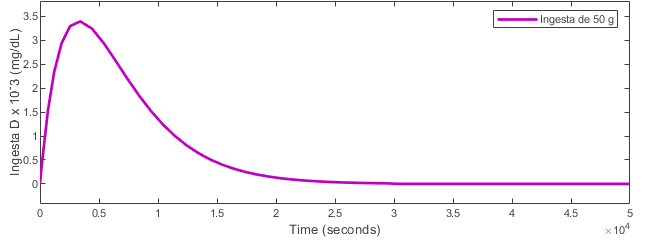
\includegraphics[width=0.9\linewidth]{img/modelo_modificado/en_metodologia/ingesta_sola.png}
    \caption{Gráfica de la ingesta D modelada según la ecuación \ref{eq:ecu_ingesta}. Fuente propia.}
    \label{fig:grafica_ingesta}
\end{figure}


\subsubsection{\underline{El ejercicio físico}}

La variable de ejercicio físico, Ej(t), ha sido incorporada en el modelo de regulación glucémica (Sección \ref{eq:glucosa_mod_mod}) para capturar los efectos de la actividad física en los niveles de glucosa en sangre. La influencia del ejercicio se refleja en la ecuación dinámica de la glucosa.  
\begin{equation} \label{eq:ejercicio_bergman}
\frac{dG(t)}{dt}= -p_1 (G(t) - G_b) - X(t)Ej(t)G(t)+D(t), G(0)=Gb 
\end{equation}
Su implementación se basa en la consideración de dos niveles de actividad física: una contribución constante durante la mayor parte del día (que representa la actividad de bajo nivel o bien la inactividad) y un período de ejercicio adicional de intensidad moderada. En los intervalos donde se produce el aumento de actividad física, se produce una contribución adicional que se suma a la contribución constante. 
La tasa de contribución constante de ejercicio al metabolismo empleada en \cite{tarin2021modelo}, es la indicada en la ecuación (\ref{eq:ejercicio_ec_bergman}) y simulada en la Figura \ref{fig:grafica_ejercicio} y se expresa en unidades de flujo por minuto. 
\begin{align} \label{eq:ejercicio_ec_bergman}
cons = 0.005/60 \\
Ej = 0.005/60 + cons,\text{si se está realizando ejercicio.}
\end{align}

\begin{figure}[htbp]
    \centering
    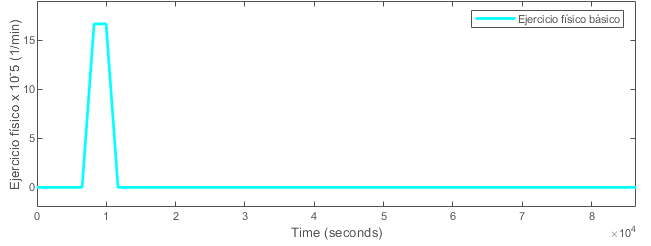
\includegraphics[width=0.9\linewidth]{img/modelo_modificado/en_metodologia/ejercicio.png}
    \caption{Gráfica de la ingesta D modelada según la ecuación \ref{eq:ejercicio_ec_bergman}. Fuente propia.}
    \label{fig:grafica_ejercicio}
\end{figure}

Se lleva a cabo una comparación entre la realización de ejercicio físico antes y después de las ingestas, basada en un estudio publicado en el American Journal of Medicine. Este estudio sugiere que la actividad física puede tener un efecto más pronunciado en la reducción de los niveles de glucosa en sangre y en la mejora de la sensibilidad a la insulina después de las comidas \footnote{Se hace referencia a este estudio específico disponible en el artículo publicado en  \cite{gwhospital_exercise_diabetes} para respaldar esta comparación.}.


\textbf{\underline{Análisis de la equivalencia funcional entre la insulina }} \\
\textbf{\underline{externa y el ejercicio}}

La actividad física regular conduce a numerosas adaptaciones en el músculo esquelético que permiten que genere ATP de manera más eficiente, siendo algunas de las adaptaciones clave una mayor absorción de glucosa y expresión de GLUT4, proteína captadora de glucosa. El entrenamiento físico aeróbico provoca la transformación del tipo de fibra muscular en un fenotipo más oxidativo y quizás más lento, y un aumento de la actividad y el contenido mitocondrial. Algunos de los efectos positivos y beneficios del ejercicio físico sobre la población diabética son la mejora de la hemoglobina glicosilada (HbA1c)\footnote{Más información en \cite{diabetes2006effects}}, reducción de la dosis diaria de insulina, mejora del perfil lipídico, disminución de retinopatías y menor incidencia de enfermedad cardiovascular. De particular importancia es la reducción de las necesidades de insulina después de realizar ejercicio. Los autores del artículo especularon que los pacientes tienden a reducir su dosis de insulina para prevenir la hipoglucemia inducida por el ejercicio. Además, el ejercicio reduce drásticamente la concentración de glucosa en sangre en un grado que depende de su intensidad, duración y el nivel concurrente de insulinemia. También aumentaría la absorción de glucosa estimulada por la insulina en el músculo, teniendo en cuenta que este efecto es mayor en el músculo entrenado que en el músculo no entrenado, lo que lleva a una reducción en el requerimiento de insulina.
Ahora bien, en el estudio \cite{salem2010exercise}, Mona A. Salem y otros demuestran que la práctica de ejercicio aeróbico moderado prolongado en pacientes diabéticos tipo 1 produce una reducción constante de la glucosa plasmática, así como la aparición de hipoglucemia si las concentraciones de glucosa antes del ejercicio son inferiores a 120 mg/dL.
En este apartado, se busca comparar la efectividad del ejercicio físico frente a la administración de insulina, así como explorar el efecto de combinar ambas intervenciones y su posible impacto en la reducción de las dosis de insulina necesarias.

\section{Control automático}

La administración de insulina exógena mediante dosis previamente estudiadas, atendiendo a los niveles basales del paciente, así como a la cantidad de ingesta que se va a producir constituye una mecánica efectiva para la estabilización de los niveles de glucosa en el organismo. Sin embargo, en ocasiones la determinación de la dosis y el momento adecuado de la administración, puede ser un desafío debido a la complejidad de las respuestas biológicas. 
Para abordar este problema, los sistemas de control automático son empleados para modelar y regular los niveles de glucosa. Uno de los enfoques ampliamente utilizados en ingeniería de control, por su efectividad y simpleza, es el regulador PID (Proporcional -Integral- Derivativo). Un controlador de este tipo se basa en el concepto de realimentación o feedback, calcula la acción de control u(t) en base al error e(t), diferencia entre el valor deseado w(t) para la variable controlada y su valor real y(t)  que se mide continuamente. Este concepto de puede observar en la Figura \ref{fig:lazo_cerrado} \footnote{Obtenida de los apuntes de la asignatura de Ingeniería de Control.}.

En el caso que nos ocupa, la referencia es el nivel concreto de glucosa en el que se quiere que esté el paciente, el error es la diferencia entre este nivel deseado y la glucosa real que tiene, y la acción de control (o variable manipulada) es la cantidad de insulina exógena que se tiene que administrar mediante la bomba de inyección.

En el caso de pacientes con diabetes tipo 1, este regulador, junto con la bomba de insulina (actuador) y el sensor de glucosa (transmisor), sustituye al comportamiento del páncreas.
\begin{figure}[htbp]
    \centering
    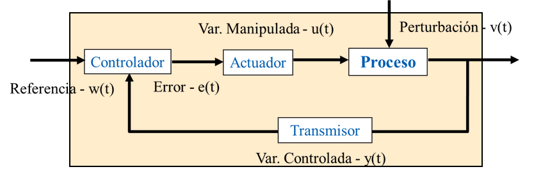
\includegraphics[width=0.9\linewidth]{img/modelo_modificado/en_metodologia/sistema en lazo cerrado.png}
    \caption{Comportamiento de un sistema en lazo cerrado. Obtenido de la asignatura de Ingeniería de Control.}
    \label{fig:lazo_cerrado}
\end{figure}

\subsection{El regulador PID}

El error, calculado como e(t) = w(t) – y(t), se incluye en la acción de control calculada de un regulador, que viene dada por la siguiente ecuación:
\begin{equation}
u(t) = Kp (e(t) + \frac{1}{Ti} \int_{0}^{t} e(\tau) \, d\tau + Td \frac{d e(t)}{dt}
\label{eq:eq_regulador}
\end{equation}
Donde se diferencian los tres términos, delimitados por signos de suma (+). Esta incluye tres parámetros fundamentales para el diseño, por orden:
\begin{enumerate}
    \item[-] Para el término proporcional, la ganancia Kp.
    \item[-] Para el término integral, el tiempo integral Ti. Ti es el tiempo que tarda la acción.
    \item[-] Para el término derivativo, el tiempo derivativo Td.
\end{enumerate}

\subsubsection{Problemática del regulador proporcional}
\label{sec:problematica_P}
Se comenzará por el regulador P, que se rige por la siguiente acción de control:
\begin{equation}
u(t) = Kp * error(t)
\label{eq:termino_P}
\end{equation}
Además, para este tipo de regulador, Kp = P (termino proporcional).

Para ciertos procesos con un regulador solo proporcional no es posible conseguir que la variable controlada alcance exactamente el valor de la referencia. Concretamente, si el error es constante, (e(t) = cte.) la acción de control u(t) es constante y no cambia más, lo que implica que la glucosa en sangre nunca se estabilice en su valor basal. E(t) se hará 0 únicamente al incluir el término integral, mediante un regulador PI.

\subsubsection{Término integral: el regulador PI}

El regulador PI adiciona a la acción de control del término proporcional P (\ref{eq:termino_P}) la siguiente acción de control:
\begin{equation}
u(t) = \frac{Kp}{Ti}\int_{0}^{t} e(\tau) \, d\tau
\label{eq:termino_I}
\end{equation}

Su relación con el término integral es: I = 1/Ti.
La idea de este tipo de regulador es calcular la acción de control u(t) de manera que si el error es constante la u(t) siga creciendo (como se observa en la ecuación (\ref{eq:termino_I})).

\subsubsection{El término derivativo D}

Debido a que un regulador P con ganancia alta para dar respuesta
rápida puede provocar oscilaciones por acción de control u excesiva, se incluye en los reguladores un nuevo término, el derivativo, cuya acción modera la u si el error decrece rápidamente, evitando estas oscilaciones. La acción derivativa se basa en la tasa de cambio del error en el tiempo, de manera que si tasa de cambio del error es alta, la acción derivativa genera una señal de control más fuerte, mientras que si la tasa de cambio es baja, la acción derivativa genera una señal más débil.

Su acción de control viene dada por la siguiente ecuación:
\begin{equation}
u(t) = Kp (e(t) + T_d \frac{d e(t)}{dt})
\label{eq:termino_d}
\end{equation}
Con esta nueva acción de control (\ref{eq:termino_d}), se consigue suavizar la respuesta de la variable controlada, pero se pueden generar cambios bruscos en la manipulada.

\subsection{Métodos de sintonía de reguladores}

El propósito de este apartado es desarrollar un modelo en Simulink que integre un regulador PID para simular el efecto de la insulina exógena en el control de los niveles de glucosa para un paciente diabético. Se emplearán métodos de sintonización sencillos para determinar los parámetros óptimos del PID.
En este contexto, se presentan dos enfoques de diseño y sintonización de reguladores. El primero es conocido como “método de prueba y error”, mientras que posteriormente se aplicará un método basado en experimentos mediante la minimización de error usando el método de López. Este método está pensado para rechazar de manera efiente las perturbaciones que afecten al proceso. En este caso, la referencia se suele mantener en el valor de la glucosa basal y lo que se pretende es mantener este nivel cuando ocurran perturbaciones como la ingesta de alimentos.

\subsubsection{Método de prueba y error}

El método basa su criterio en una estimación manual de los parámetros proporcionales e integrales del regulador. De esta forma, se parte de un valor bajo para Kp, sin acción integral ni derivativa, hasta obtener una respuesta integrada en el modelo simulado que sea similar al comportamiento de dicho modelo con una entrada de insulina exógena. Una vez realizado esto, se van modificando los valores de Ti y Td hasta lograr el comportamiento óptimo.


Se pretende demostrar, que, pese a la sencillez de implementación de este método de sintonía, la selección del valor adecuado de los parámetros es clave para el correcto funcionamiento del regulador, haciendo que una leve variación de ellos puede provocar comportamientos que supongan riesgos considerables para la estabilidad el paciente.

\subsubsection{Método basado en experimentos}

Este enfoque se basa en la realización de un experimento de salto en la entrada del sistema (en este caso, la insulina exógena) y la observación de la respuesta del sistema. Uno de los métodos ampliamente utilizados en este contexto es el Método de López, que proporciona una manera sistemática de derivar los parámetros del PID a partir de la respuesta transitoria del sistema considerando el rechazo de perturbaciones.
Este procedimiento de identificación aproxima la respuesta del proceso en lazo abierto por un sistema de primer orden con retardo, representado por la siguiente función de transferencia:
\begin{equation}
G(s) = \frac{K e^{-ds}}{\tau s +1}
\label{eq:sist_primer_o_retardo}
\end{equation}
Donde K es la ganancia, tau la constante de tiempo, y d el retardo. El cálculo de estos parámetros es necesario para la posterior obtención de los términos proporcional, integral y derivativo. Para ello, inicialmente, es necesario modelar este sistema de primer orden.
Se parte de una situación de estabilidad, en la cual, si el paciente no recibe ingestas, sus niveles de glucosa permanecen constantes gracias a la administración de insulina. Esta cantidad ha sido calculada ya en la Sección \ref{sec:dosis_insu_base}. 
A continuación, se varía el modelo para una entrada escalón de insulina, pasando de la U inicial a otra cantidad mayor de insulina. Ante esta situación, el modelo ya nos puede aportar la información necesaria para obtener los parámetros solicitados, que son:

\begin{align}
\tau = 1.5 (t2-t1) \\
d = t2- \tau \\
K= \frac{\delta y}{\delta u} \\
\label{eq:sist_primer_o_retardo}
\end{align}

Una vez obtenidos K, tau y d, se halla el valor de Kp y Ti, para lograr así obtener el valor de los términos proporcional e integral, siguiendo la misma consideración que con el método anterior, donde Kp = P, I = 1/Ti. Este cálculo se realizará mediante el método de López, que minimiza la integral del error, y es válido para procesos monótonos con d/tau <1. 
Se especifica además uno de los criterios basados en toda la respuesta, el criterio MITAE, por ser el más suavizado, cuyos valores se encuentran en las tablas \ref{tab:valores_PI_MITAE} y \ref{tab:valores_PID_MITAE}.
\begin{table}[htbp]
    \centering
    \caption{Valores de a, b para un PI con el criterio MITAE.}
    \begin{tabular}{|c|c|c|}
        \hline
        Proporcional & Integral  \\
        \hline
        a = 0.859 & a = 0.674\\
        b = -0.977 & b = -0.68\\
        \hline
    \end{tabular}
    \label{tab:valores_PI_MITAE}
\end{table}
\begin{table}[htbp]
    \centering
    \caption{Valores de a, b para un PID con el criterio MITAE.}
    \begin{tabular}{|c|c|c|}
        \hline
        Proporcional & Integral & Derivativo  \\
        \hline
        a = 1.357 & a = 0.842 & a = 0.381\\
        b = -0.947 & b = -0.738& b = -0.995\\
        \hline
    \end{tabular}
    \label{tab:valores_PID_MITAE}
\end{table}

Así, se despejan de las siguientes ecuaciones Kp y Ti:
\begin{align}
Kp K = a (\frac{d}{\tau})^b \\
\frac{\tau}{Ti} = a (\frac{d}{\tau})^b \\
\frac{Td}{\tau} = a (\frac{d}{\tau})^b \\
\label{eq:lopez}
\end{align}


\section{Técnicas y herramientas}

\subsection{MatLab}
MATLAB \cite{matlab2021matlab} es una plataforma de programación y cálculo numérico utilizada para analizar datos, desarrollar algoritmos y crear modelos. Es la abreviatura de MATrix LABoratory y ofrece un entorno de desarrollo integrado (IDE) con un lenguaje de programación propio. Se encuentra disponible para los sistemas operativos Windows, Unix, GNU/Linux y macOS. Puesto que se trata de un lenguaje con base en scripts, la creación de programas y su depuración en MATLAB con frecuencia es más fácil que en los lenguajes de programación tradicionales, como C++. MATLAB ofrece una extensa biblioteca de funciones predefinidas para realizar una variedad de tareas técnicas, siendo ampliamente empleado en campos como la ingenería.
\subsection{SIMULINK}

Simulink es una herramienta de simulación y modelado dinámico que se integra con MATLAB. Este entorno de diagramas de bloque, se utiliza para diseñar sistemas con modelos multidominio, simular antes de implementar en hardware y desplegar sin necesidad de escribir código. Simulink es particularmente útil para simular y analizar sistemas de control, sistemas de potencia, sistemas de comunicación y otros sistemas dinámicos. Además,  también ofrece capacidades de simulación avanzadas y herramientas de análisis para evaluar el rendimiento del sistema y optimizar el diseño del modelo.

\subsection{LaTex}
LaTeX \cite{latexweb} es un sistema tipográfico de alta calidad que incluye funcionalidades diseñadas para la producción de documentación técnica y científica. LaTeX es el estándar de facto para la comunicación y publicación de documentos científicos y está disponible como software gratuito. Para la realización del trabajo se emplea Overleaf, un editor LaTeX colaborativo en tiempo real, en línea y de código abierto. Para más información de este herramienta, consultar el repositorio de GitHub  \cite{overleafgithub}.


